\documentclass[aspectratio=169]{../latex_main/tntbeamer}  % you can pass all options of the beamer class, e.g., 'handout' or 'aspectratio=43'
\usepackage{dsfont}
\usepackage{bm}
\usepackage[english]{babel}
\usepackage[T1]{fontenc}
%\usepackage[utf8]{inputenc}
\usepackage{graphicx}
\graphicspath{ {./figures/} }
\usepackage{algorithm}
\usepackage[ruled,vlined,algo2e,linesnumbered]{algorithm2e}
\usepackage{hyperref}
\usepackage{booktabs}
\usepackage{mathtools}

\usepackage{amsmath,amssymb}

\DeclareMathOperator*{\argmax}{arg\,max}
\DeclareMathOperator*{\argmin}{arg\,min}

\usepackage{pgfplots}
\pgfplotsset{compat=1.16}
\usepackage{tikz}
\usetikzlibrary{trees} 
\usetikzlibrary{shapes.geometric}
\usetikzlibrary{positioning,shapes,shadows,arrows,calc,mindmap}
\usetikzlibrary{positioning,fadings,through}
\usetikzlibrary{decorations.pathreplacing}
\usetikzlibrary{intersections}
\pgfdeclarelayer{background}
\pgfdeclarelayer{foreground}
\pgfsetlayers{background,main,foreground}
\tikzstyle{activity}=[rectangle, draw=black, rounded corners, text centered, text width=8em]
\tikzstyle{data}=[rectangle, draw=black, text centered, text width=8em]
\tikzstyle{myarrow}=[->, thick, draw=black]

% Define the layers to draw the diagram
\pgfdeclarelayer{background}
\pgfdeclarelayer{foreground}
\pgfsetlayers{background,main,foreground}

% Requires XeLaTeX or LuaLaTeX
\usepackage{unicode-math}

\usepackage{fontspec}
%\setsansfont{Arial}
\setsansfont{RotisSansSerifStd}[ 
Path=../latex_main/fonts/,
Extension = .otf,
UprightFont = *-Regular,  % or *-Light
BoldFont = *-ExtraBold,  % or *-Bold
ItalicFont = *-Italic
]
\setmonofont{Cascadia Mono}[
Scale=0.8
]

% scale factor adapted; mathrm font added (Benjamin Spitschan @TNT, 2021-06-01)
%\setmathfont[Scale=1.05]{Libertinus Math}
%\setmathrm[Scale=1.05]{Libertinus Math}

% other available math fonts are (not exhaustive)
% Latin Modern Math
% XITS Math
% Libertinus Math
% Asana Math
% Fira Math
% TeX Gyre Pagella Math
% TeX Gyre Bonum Math
% TeX Gyre Schola Math
% TeX Gyre Termes Math

% Literature References
\newcommand{\lit}[2]{\href{#2}{\footnotesize\color{black!60}[#1]}}

%%% Beamer Customization
%----------------------------------------------------------------------
% (Don't) Show sections in frame header. Options: 'sections', 'sections light', empty
\setbeamertemplate{headline}{empty}

% Add header logo for normal frames
\setheaderimage{
	% 
\includegraphics[height=\logoheight]{figures/TNT_darkv4.pdf}
	
\includegraphics[height=\logoheight]{../latex_main/figures/luh_logo_rgb_0_80_155.pdf}
	% 
\includegraphics[height=\logoheight]{figures/logo_tntluh.pdf}
}

% Header logo for title page
\settitleheaderimage{
	% 
\includegraphics[height=\logoheight]{figures/TNT_darkv4.pdf}
	
\includegraphics[height=\logoheight]{../latex_main/figures/luh_logo_rgb_0_80_155.pdf}
	% 
\includegraphics[height=\logoheight]{figures/logo_tntluh.pdf}
}

% Title page: tntdefault 
\setbeamertemplate{title page}[tntdefault]  % or luhstyle
% Add optional title image here
%\addtitlepageimagedefault{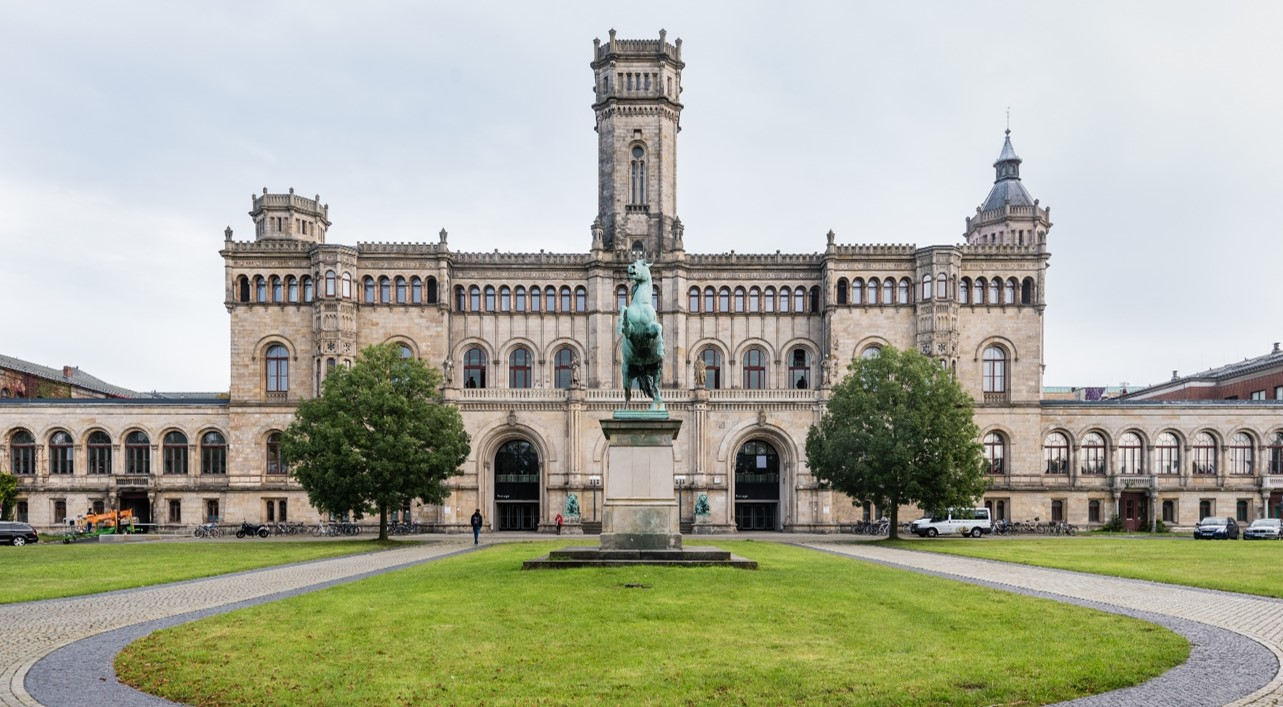
\includegraphics[width=0.65\textwidth]{figures/luh_default_presentation_title_image.jpg}}

% Title page: luhstyle
% \setbeamertemplate{title page}[luhstyle]
% % Add optional title image here
% \addtitlepageimage{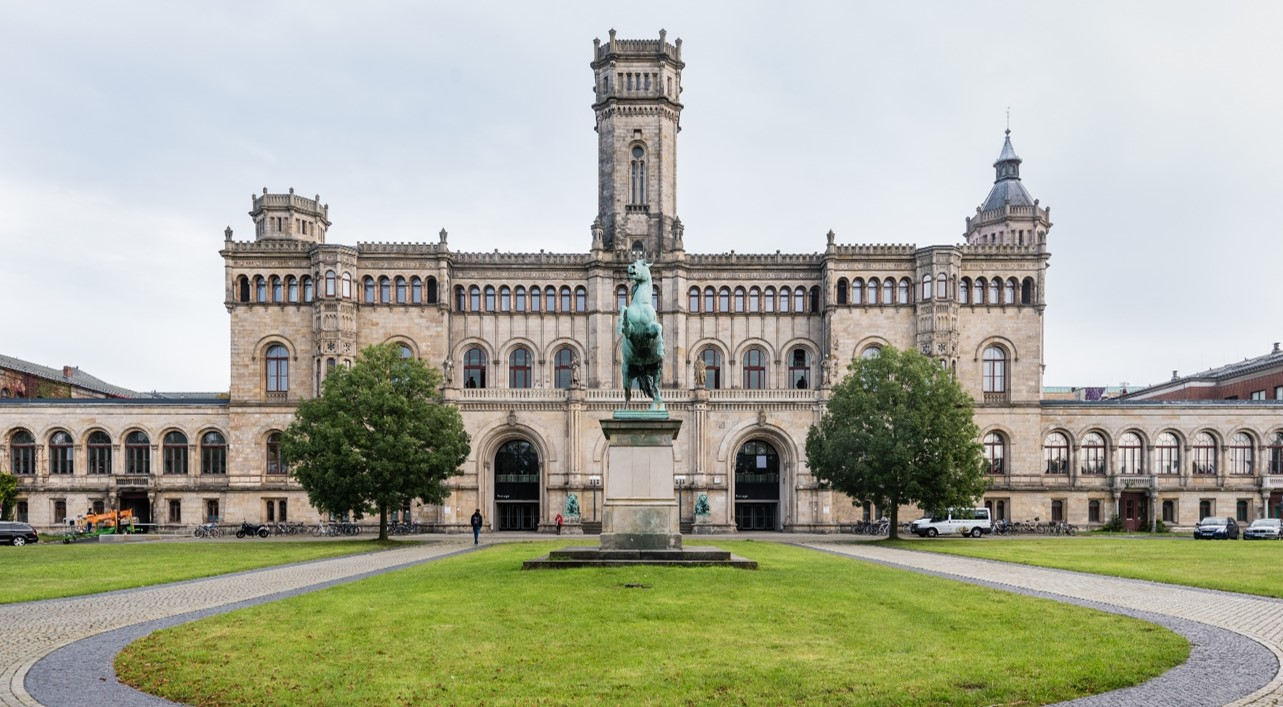
\includegraphics[width=0.75\textwidth]{figures/luh_default_presentation_title_image.jpg}}

\author[Lindauer \& Anand]{Marius Lindauer and Avishek Anand\\[1em]
	
\includegraphics[height=\logoheight]{../latex_main/figures/luh_logo_rgb_0_80_155.pdf}\qquad

\includegraphics[height=\logoheight]{../latex_main/figures/TNT_darkv4}\qquad

\includegraphics[height=\logoheight]{../latex_main/figures/L3S.jpg}	}
\date{Winter Term 2021
}


%%% Custom Packages
%----------------------------------------------------------------------
% Create dummy content
\usepackage{blindtext}

% Adds a frame with the current page layout. Just call \layout inside of a frame.
\usepackage{layout}


\title[Introduction]{iML: Introduction}
\subtitle{Motivating Examples}

%\institute{}


\begin{document}
	
	\maketitle

\begin{frame}[c]{Why is Interpretability Important?}
	
	\begin{itemize}
	    \item Machine learning is (mostly) about discovering patterns in data
	    \item Unfortunately, it is not guaranteed that ML will identify the correct patterns
	    \pause
	    \medskip
	    \item We humans might not be able to discover patterns ML models discovered
	    \begin{itemize}
	        \item That's good for science or to get new insights
	        \item That's bad in many practical application where unexpected behavior is not wanted
	    \end{itemize}
	    \medskip
	    \pause
	    \item \alert{How can you check whether the model is correct in its inference?}
	\end{itemize}
	
\end{frame}

\begin{frame}[c]{Clever Hans \lit{Lapuschkin et al. 2019}{https://www.nature.com/articles/s41467-019-08987-4}}
	
	\centering
	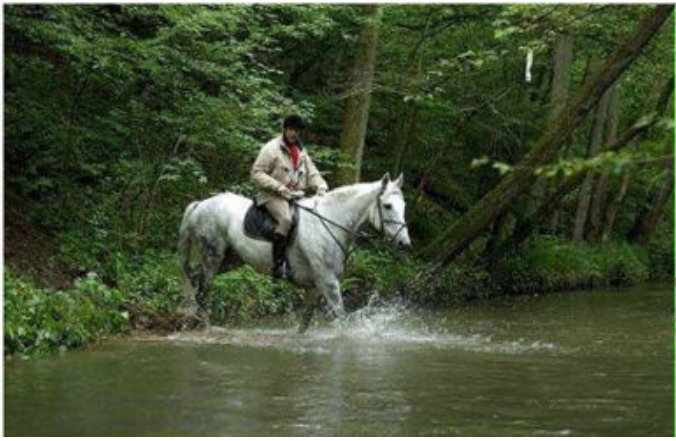
\includegraphics[width=0.6\textwidth]{./figure/horse_without_label.PNG}
	
\end{frame}

\begin{frame}[c]{Clever Hans \lit{Lapuschkin et al. 2019}{https://www.nature.com/articles/s41467-019-08987-4}}
	
	\centering
	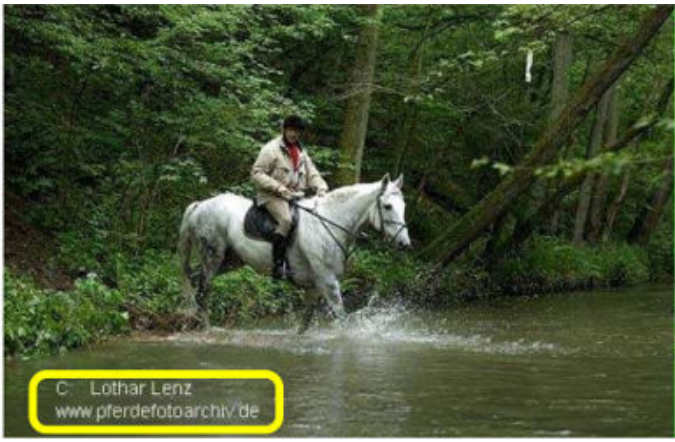
\includegraphics[width=0.6\textwidth]{./figure/horse_with_label.PNG}
	
\end{frame}

\begin{frame}[c]{Clever Hans \lit{Lapuschkin et al. 2019}{https://www.nature.com/articles/s41467-019-08987-4}}
	
	\centering
	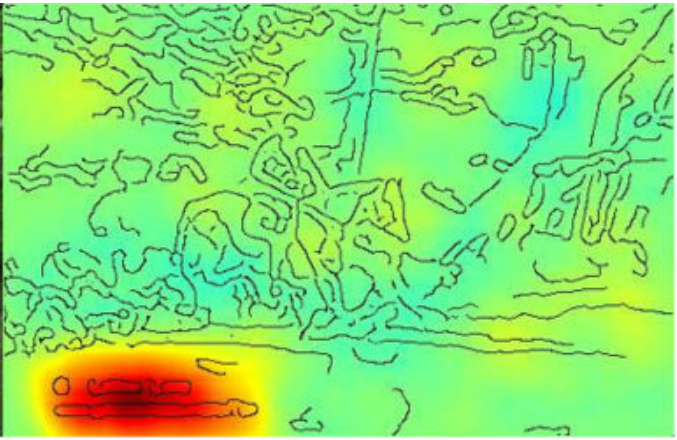
\includegraphics[width=0.6\textwidth]{./figure/horse_map_with_label.PNG}
	
\end{frame}

\begin{frame}[c]{Clever Hans \lit{Lapuschkin et al. 2019}{https://www.nature.com/articles/s41467-019-08987-4}}
	
	\centering
	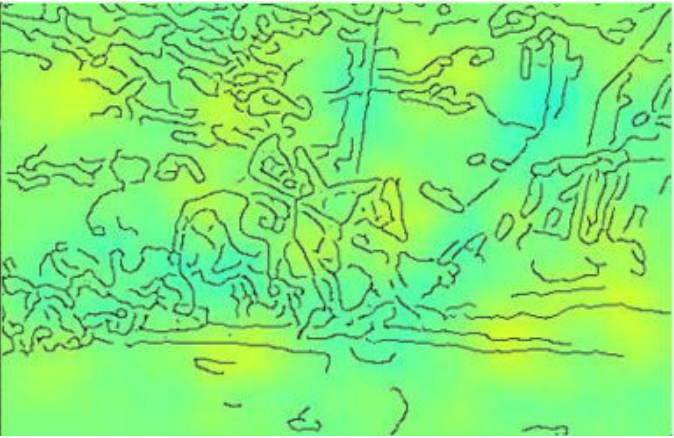
\includegraphics[width=0.6\textwidth]{./figure/horse_map_without_label.PNG}
	
\end{frame}

\begin{frame}[c]{Clever Hans \lit{Lapuschkin et al. 2019}{https://www.nature.com/articles/s41467-019-08987-4}}
	
	\centering
	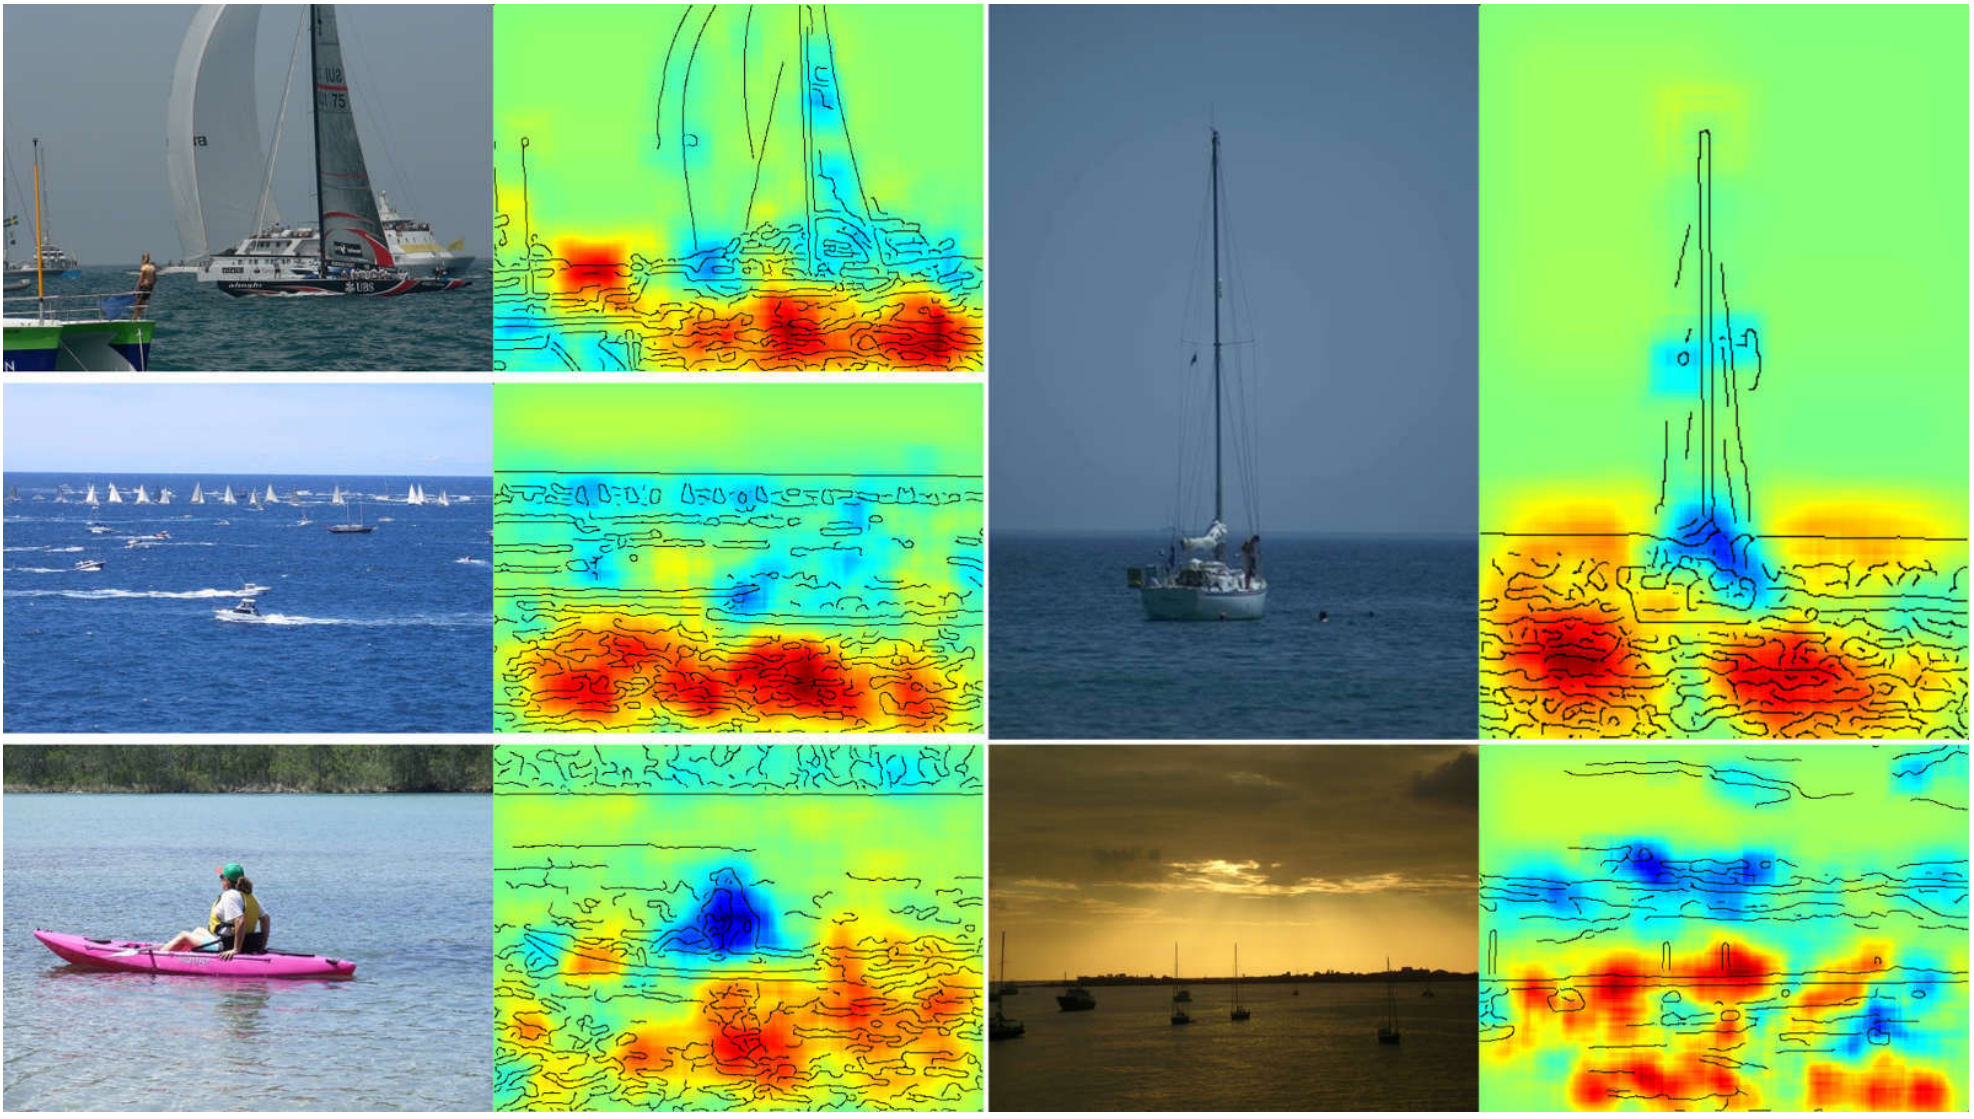
\includegraphics[width=0.6\textwidth]{./figure/boats_maps.PNG}
	
\end{frame}

\begin{frame}[c]{COMPASS}

    \begin{itemize}
        \item Correctional Offender Management Profiling for Alternative Sanctions 
        \item predict recidivism risk
        \begin{itemize}
            \item i.e., criminal re-offense after previous crime, resulting in jail booking
            \item different risk levels: high risk, medium risk or low risk
        \end{itemize}
        \item evaluation based on a questionnaire the defendant has to answer
    \end{itemize}	
	
\end{frame}

\begin{frame}[c]{COMPAS Model Analysis~\lit{Larson et al. 2016}{https://www.propublica.org/article/how-we-analyzed-the-compas-recidivism-algorithm}}
    
    \centering
    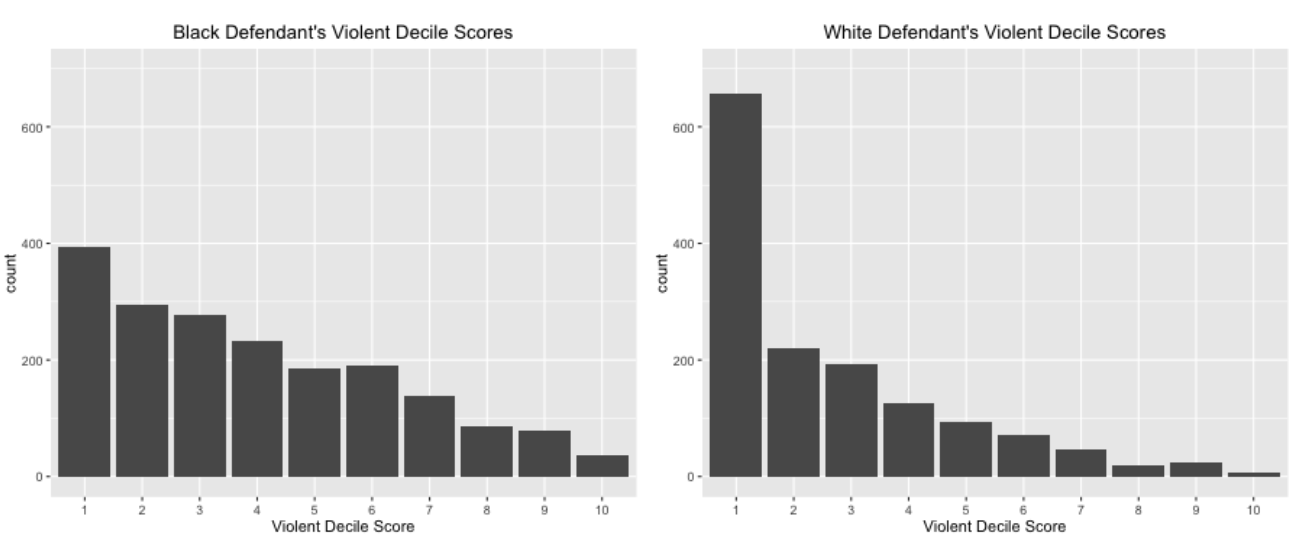
\includegraphics[width=0.7\textwidth]{./figure/compass_black_white.PNG}
	
	$\leadsto$ Strong indication that the model is discriminating black defendants
	
\end{frame}

\begin{frame}[c]{Other Examples ML failed in}

    \begin{itemize}
        \item Credit and insurance scoring
        \pause
        \item Medical applications
        \begin{itemize}
            \item Identification of diseases
            \item Chance of recovering
            \item Recommendations of treatments
        \end{itemize}
        \pause
        \item Crime predictions
        \pause
        \item Rating job applications
        \pause
        \item \ldots
    \end{itemize}

    \pause
    \bigskip

    $\leadsto$ GDPR (aka DSGVO) requires that for some applications predictive models have to be explainable        
	
\end{frame}



\begin{frame}[c]{Adversarial Examples~\lit{Goodfellow et al. 2016}{https://arxiv.org/pdf/1412.6572.pdf}}
    
    \centering
    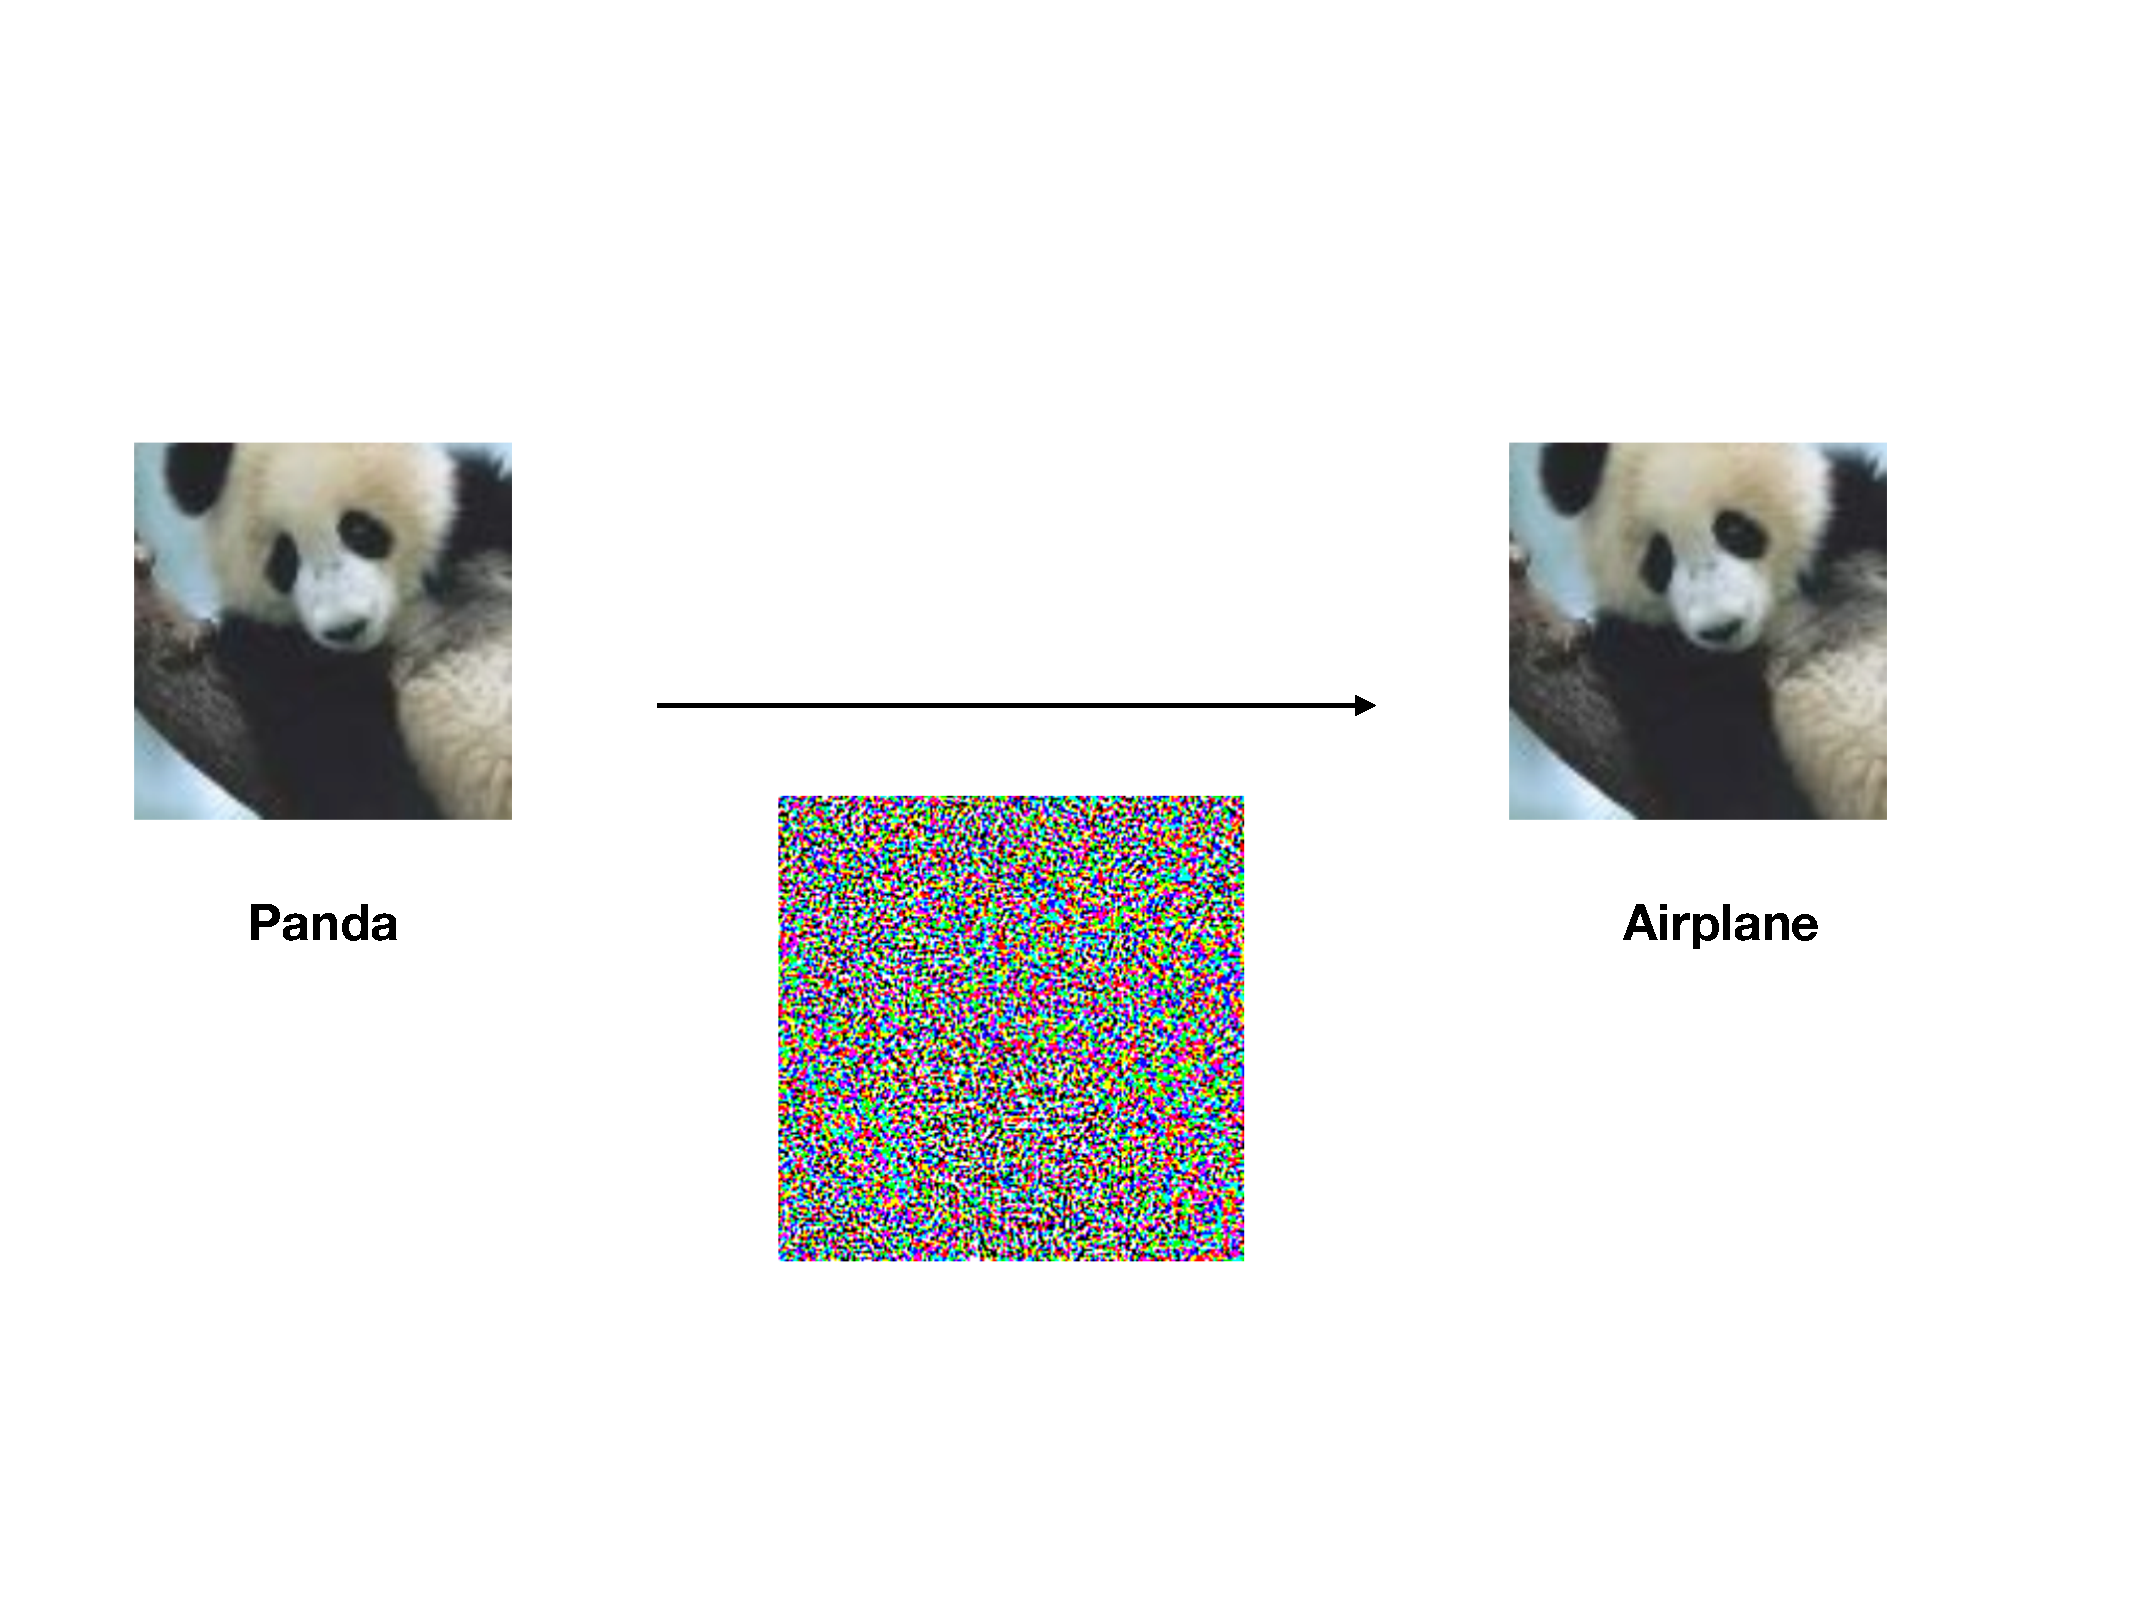
\includegraphics[width=0.7\textwidth]{./figure/panda-airplane.pdf}
	
	$\leadsto$ ML Models might not capture human-like understanding.        
	
\end{frame}

	
\begin{frame}[c]{Adversarial Noise~\lit{Goodfellow et al. 2016}{https://arxiv.org/pdf/1412.6572.pdf}}
    
    \centering
    \includegraphics[width=0.6\textwidth]{./figure/adv-noise.pdf}
	
	$\leadsto$ \textbf{Adversarial Noise:} Noise that is imperceptible to \textbf{humans}\\ but results in incorrect classification results
	
\end{frame}

\begin{frame}[c]{Adversarial Examples~\lit{Goodfellow et al. 2016}{https://arxiv.org/pdf/1412.6572.pdf}}
    
    \centering
    \includegraphics[width=0.7\textwidth]{./figure/adv-noise-2.pdf}
	
\end{frame}

\end{document}
